\documentclass{article}

\usepackage{cmap}
\usepackage{amsmath,amsthm,amssymb}
\usepackage[T1]{fontenc}
\usepackage[utf8]{inputenc}
\usepackage[english]{babel}
\usepackage{lmodern}
\usepackage{microtype}
\usepackage{graphicx}
\usepackage{hyperref}
\usepackage{booktabs}
\usepackage{array}

\title{A Reproducible Benchmark for OCR Post-Correction of Low-Resource Arabic-Script Turkic Historical Texts}
\author{Radmir}
\date{Spring 2026}

\begin{document}
\maketitle

\begin{abstract}
This project studies OCR post-correction for historical Turkic texts written in Arabic script. We formulate the problem as a sequence-to-sequence NLP task: given a noisy OCR-like text line, the system should generate its clean version. We collect a small Arabic-script Turkic corpus, construct a synthetic noisy-clean benchmark, compare identity and rule-based baselines with a ByT5-small model, and evaluate the results with Character Error Rate (CER), Word Error Rate (WER), and Exact Match. On the proposed benchmark, ByT5-small with a 512-token sequence length achieves the best CER and WER among the evaluated methods. The project code is available at: \url{https://github.com/Therad445/low-resource-arabic-script-turkic-ocr}.
\end{abstract}

\section{Introduction}

Historical Turkic texts written in Arabic script are important for linguistic, cultural and historical research. However, such materials remain difficult to process automatically. The task is low-resource: there are few annotated corpora, orthography is unstable, document quality varies, and standard OCR and NLP tools are usually designed for modern high-resource languages and scripts.

This project focuses on OCR post-correction. We do not attempt to solve full image-based OCR or handwritten text recognition. Instead, we isolate the next NLP stage: correcting an already produced noisy text output. The task is formulated as:
\[
\text{noisy Arabic-script Turkic text} \rightarrow \text{clean Arabic-script Turkic text}.
\]

The main contributions are:
\begin{itemize}
    \item a small reproducible benchmark for Arabic-script Turkic OCR post-correction;
    \item a synthetic OCR-like noise generation protocol;
    \item a clean-line-level train/validation/test split without leakage;
    \item comparison of identity, rule-based and neural sequence-to-sequence approaches;
    \item evaluation with CER, WER and Exact Match;
    \item per-sample error analysis of model improvements and degradations.
\end{itemize}

\subsection{Team}

\textbf{Radmir} collected and prepared the corpus, constructed the synthetic post-correction dataset, implemented and evaluated the baselines, trained and evaluated the ByT5-small model, performed error analysis, prepared the repository and wrote the final report.


\section{Related Work}
\label{sec:related}

\subsection{Historical OCR and HTR Workflows}

OCR for historical documents differs from OCR for modern clean printed text. Historical material often contains unstable typography, damaged scans, non-standard spelling, complex layouts and domain-specific writing conventions. OCR workflows for historical printings therefore usually include data preparation, ground-truth construction, model training, post-processing and manual validation \cite{reul2019ocr4all,springmann2018ocr}. These works are important for this project because they show that OCR quality is not only a model problem: it depends on data preparation, segmentation, document layout, transcription conventions and downstream correction.

This project is narrower than a full OCR or HTR workflow. It does not train an image-to-text recognizer. Instead, it isolates the post-correction stage and asks whether a text-to-text model can improve noisy OCR-like output for Arabic-script Turkic historical text.

\subsection{Arabic-Script OCR}

Arabic-script OCR is challenging because letters change shape depending on their position, the script is cursive, and many characters differ only by small dots or diacritics. These problems become stronger in historical or multilingual contexts, where Arabic, Persian and Turkic orthographic traditions can overlap. Earlier surveys emphasize such script-specific difficulties \cite{naz2014arabicocr}. More recent work on open-source Arabic-script OCR shows that accuracy depends strongly on training data, script coverage, line segmentation, layout analysis and the treatment of error patterns \cite{kiessling2024arabicocr}.

This motivates two design choices in the present project. First, the benchmark explicitly keeps Arabic-script characters rather than transliterating the data into Latin script. Second, the dataset analysis reports a character inventory and a taxonomy of synthetic OCR-like corruptions, because Arabic-script post-correction should not be evaluated only as generic text normalization.

\subsection{OCR Post-Correction Approaches}

OCR post-correction transforms noisy OCR output into a cleaner textual representation. At the line level, it can be formulated as a sequence-to-sequence problem. Quality is commonly evaluated with edit-distance-based metrics such as CER and WER, which are based on insertions, deletions and substitutions \cite{levenshtein1966binary}.

Several families of approaches exist. Rule-based and normalization-based systems are simple and interpretable, but they can be too aggressive when historical spelling variation is meaningful. Lexicon-based and edit-distance-based methods can help when a reliable vocabulary exists, but they are less suitable for low-resource historical corpora with unstable spelling. Neural post-correction methods learn character-level or sequence-level transformations from noisy-clean pairs. Lyu et al. \cite{lyu2021neural} proposed a neural approach for historical OCR post-hoc correction using character-level modelling and attention. Hamalainen and Hengchen \cite{hamalainen2019paft} and Duong et al. \cite{duong2020unsupervised} studied unsupervised extraction of parallel data for character-based sequence-to-sequence correction and spelling normalisation in historical corpora.

Compared with these works, this project is smaller in scale but targets a rarer setting: Arabic-script Turkic historical text. The benchmark is also designed to be reproducible within a course project repository.

\subsection{Low-Resource and Synthetic-Data Settings}

A recurring difficulty in OCR post-correction is the lack of manually aligned noisy-clean data. This is especially severe for historical documents and low-resource languages. Suissa et al. \cite{suissa2023optimizing} show that OCR correction for historical Hebrew benefits from task-specific training data and that correction quality depends on genre and domain. Naiman et al. \cite{naiman2023large} use synthetic ground-truth/OCR data for post-correction of historical scientific articles, demonstrating that synthetic noisy-clean pairs can be a practical way to construct large training resources when direct aligned OCR correction data is limited.

The present project follows the same general motivation, but at a smaller pilot scale. Synthetic corruption is not treated as a perfect substitute for real OCR output. Instead, it is used to build a controlled benchmark that can be extended later with real OCR or HTR predictions.

\subsection{Transformer and Byte-Level Models}

Transformer models \cite{vaswani2017attention} and text-to-text transfer learning \cite{raffel2020exploring} provide a general framework for sequence-to-sequence NLP tasks. In this project, the main neural model is ByT5 \cite{xue2022byt5}, a byte-level sequence-to-sequence model. Byte-level modelling is useful for noisy and low-resource settings because it avoids dependence on a fixed word or subword vocabulary. This is especially relevant for historical Arabic-script Turkic text, where rare spellings, mixed orthographic conventions and OCR-like distortions can make subword tokenization fragile.

Recent work has also explored large and multimodal language models for historical OCR and post-correction. Greif et al. \cite{greif2025multimodal} study multimodal LLMs for OCR, OCR post-correction and named entity recognition in historical documents. Such approaches are promising, but they often require large proprietary models or image-based inputs. The present project instead uses a lightweight, reproducible fine-tuning setup on text-level noisy-clean pairs.

\subsection{Positioning of This Work}

Table~\ref{tab:related-work} summarizes the most relevant previous work and how it relates to this project. The main difference is that this project focuses on a small but explicit Arabic-script Turkic post-correction benchmark, with controlled synthetic noise, leakage-safe splits, baseline comparisons and error analysis.

\begin{table}[tbh!]
\begin{center}
\scriptsize

\begin{tabular}{p{0.17\linewidth}p{0.14\linewidth}p{0.18\linewidth}p{0.20\linewidth}p{0.20\linewidth}}
\toprule
Work & Setting & Method & Main contribution & Relation to this project \\
\midrule
OCR4all \cite{reul2019ocr4all} & Historical printings & OCR workflow & Semi-automatic OCR workflow with ground-truth preparation and model training & Motivates the full historical OCR pipeline; this project focuses only on post-correction \\
Springmann et al. \cite{springmann2018ocr} & Historical printings & OCR and corpus construction & Shows how historical OCR supports diachronic corpora & Provides historical OCR context and the need for downstream correction \\
Lyu et al. \cite{lyu2021neural} & Historical German corpora & Neural post-correction & Character-level neural correction for historical OCR output & Closest neural post-correction baseline in spirit, but not Arabic-script or Turkic \\
Hamalainen and Hengchen \cite{hamalainen2019paft} & Historical corpora & Unsupervised NMT & Automatically extracts parallel data for character-level NMT correction & Alternative to our supervised synthetic noisy-clean benchmark \\
Duong et al. \cite{duong2020unsupervised} & Finnish historical corpora & Unsupervised seq2seq & Combines OCR correction with spelling normalisation & Shows low-resource post-correction without manual parallel data \\
Suissa et al. \cite{suissa2023optimizing} & Historical Hebrew & Neural OCR correction & Studies task-specific training data and genre effects & Supports our focus on script-specific and corpus-specific error modelling \\
Naiman et al. \cite{naiman2023large} & Historical scientific articles & Synthetic OCR data & Builds a large synthetic ground-truth OCR post-correction dataset & Justifies synthetic noisy-clean pairs as a practical benchmark strategy \\
Kiessling et al. \cite{kiessling2024arabicocr} & Arabic-script OCR & Kraken OCR study & Provides Arabic-script OCR evaluation and error microanalysis & Directly motivates Arabic-script error analysis and training-data sensitivity \\
ByT5 \cite{xue2022byt5} & Multilingual NLP & Byte-level Transformer & Avoids subword tokenization and improves robustness to noise & Main model choice for noisy Arabic-script post-correction \\
Greif et al. \cite{greif2025multimodal} & Historical documents & Multimodal LLMs & Uses mLLMs for OCR, post-correction and NER & Recent frontier approach; our work is lighter and reproducible without mLLM APIs \\
\bottomrule
\end{tabular}

\caption{Comparison with related work on historical OCR, Arabic-script OCR and OCR post-correction.}
\label{tab:related-work}
\end{center}
\end{table}


\section{Model Description}

The project compares three approaches.

\subsection{Identity Baseline}

The identity baseline returns the noisy input unchanged. It measures the initial quality of the synthetic OCR-like text and serves as the simplest reference point.

\subsection{Rule-Based Normalizer}

The rule-based normalizer applies simple Arabic-script normalization rules. This baseline tests whether naive character normalization is useful for this material. Since historical orthography may contain meaningful variation, aggressive normalization can be harmful.

\subsection{ByT5-small}

The main neural approach is ByT5-small. It is fine-tuned as a sequence-to-sequence model. The input is a noisy OCR-like line, and the target is the corresponding clean line. The final evaluated configuration uses 512-token source and target sequence lengths and is trained for 2 epochs.

The use of a byte-level model is motivated by the low-resource and noisy nature of the task. Arabic-script characters may occupy multiple bytes, and historical spelling variation can be poorly represented by standard subword tokenizers. Therefore, sequence length is an important experimental parameter.



\section{Dataset}

The dataset is a pilot benchmark for OCR post-correction of Arabic-script Turkic historical text. The clean corpus was collected from an Ottoman Turkish / Arabic-script Turkic Wikisource source. The project does not use document images directly at this stage; instead, it isolates the text-level post-correction problem by generating synthetic OCR-like noisy versions of clean historical lines.

\subsection{Corpus Structure and Splits}

Each processed CSV file contains four fields:
\begin{itemize}
    \item \texttt{line\_id}: identifier of the original clean line;
    \item \texttt{variant\_id}: identifier of the synthetic noisy variant;
    \item \texttt{noisy}: synthetically corrupted OCR-like text;
    \item \texttt{clean}: original clean text.
\end{itemize}

The split is performed by clean source lines, not by individual noisy variants. This prevents leakage: noisy variants of the same original line do not appear in different splits. This is important because otherwise the model could see almost identical versions of the same clean line during training and testing. The source description is stored in \texttt{data/postcorrection/raw/SOURCES.md}. The benchmark is suitable for controlled comparison of post-correction methods, although it does not replace evaluation on real OCR or HTR output.

\begin{table}[tbh!]
\begin{center}
\begin{tabular}{lrrrr}
\toprule
Split & Clean lines & Noisy-clean pairs & Avg. clean chars & Avg. noisy chars \\
\midrule
train & 320 & 6400 & 113.94 & 113.51 \\
valid & 40 & 800 & 112.75 & 112.24 \\
test & 40 & 800 & 122.25 & 121.70 \\
\bottomrule
\end{tabular}

\caption{Dataset split statistics for the proposed Arabic-script Turkic OCR post-correction benchmark.}
\label{tab:dataset}
\end{center}
\end{table}

\subsection{Corpus Length and Character Statistics}

Table~\ref{tab:length-stats} gives a more detailed view of the corpus. The test split contains 800 noisy-clean pairs derived from 40 unique clean lines. The lines are relatively long for exact sequence-level correction: the average clean test line has more than 120 characters and about 18 words. This helps explain why Exact Match remains low even when CER and WER improve.

\begin{table}[tbh!]
\begin{center}
\small
\begin{tabular}{lrrrrrr}
\toprule
Split & Pairs & Clean lines & Avg chars & Median & Range & Avg words \\
\midrule
train & 6400 & 320 & 113.94 & 115.5 & 35--180 & 17.19 \\
valid & 800 & 40 & 112.75 & 120.0 & 41--174 & 17.15 \\
test & 800 & 40 & 122.25 & 122.0 & 39--178 & 18.18 \\
\bottomrule
\end{tabular}

\caption{Length statistics for the processed noisy-clean splits.}
\label{tab:length-stats}
\end{center}
\end{table}

The corpus contains a mixed Arabic-script character inventory. Table~\ref{tab:char-inventory} summarizes the number of characters, while Table~\ref{tab:top-chars} reports the most frequent non-space Unicode code points in the clean text. Unicode codes are used to keep the PDF stable and to make the character inventory unambiguous.

\begin{table}[tbh!]
\begin{center}
\begin{tabular}{lrr}
\toprule
Statistic & Clean text & Noisy text \\
\midrule
Total characters & 917200 & 913612 \\
Unique characters & 114 & 114 \\
\bottomrule
\end{tabular}

\caption{Character inventory summary for clean and noisy text.}
\label{tab:char-inventory}
\end{center}
\end{table}

\begin{table}[tbh!]
\begin{center}
\small
\begin{tabular}{lrr}
\toprule
Unicode code & Count & Share \\
\midrule
U+0627 & 97780 & 10.66\% \\
U+0631 & 62620 & 6.83\% \\
U+0648 & 61480 & 6.70\% \\
U+0646 & 52940 & 5.77\% \\
U+0644 & 48840 & 5.32\% \\
U+06CC & 46360 & 5.05\% \\
U+062F & 41660 & 4.54\% \\
U+064A & 34760 & 3.79\% \\
U+0647 & 34660 & 3.78\% \\
U+0645 & 34440 & 3.75\% \\
U+062A & 32740 & 3.57\% \\
U+0642 & 25140 & 2.74\% \\
\bottomrule
\end{tabular}

\caption{Most frequent non-space Unicode code points in the clean corpus.}
\label{tab:top-chars}
\end{center}
\end{table}

\subsection{Synthetic OCR-like Noise}

The benchmark uses synthetic noise to simulate common text-level OCR errors. The noise generator is intended to create a controlled post-correction benchmark rather than a fully realistic OCR system. Table~\ref{tab:noise-taxonomy} summarizes the main types of corruptions represented by the generator and observed in the noisy-clean pairs.

\begin{table}[tbh!]
\begin{center}
\small
\begin{tabular}{p{0.22\linewidth}p{0.32\linewidth}p{0.34\linewidth}}
\toprule
Noise type & Description & Motivation \\
\midrule
Character substitution & A character is replaced by another visually or script-related character. & Models OCR confusions between similar Arabic-script shapes. \\
Character deletion & A character is removed from the clean line. & Models missed glyphs, weak ink, scan noise, or segmentation loss. \\
Character insertion & An extra character is inserted into the line. & Models spurious OCR glyphs and over-segmentation. \\
Whitespace split/merge & Spaces may be inserted inside words or removed between tokens. & Models word-boundary errors in cursive OCR. \\
Arabic/Persian form confusion & Alternative forms of related Arabic-script characters are introduced. & Models mixed Arabic, Persian and Ottoman conventions. \\
\bottomrule
\end{tabular}

\caption{Synthetic OCR-like noise taxonomy used in the benchmark.}
\label{tab:noise-taxonomy}
\end{center}
\end{table}

Table~\ref{tab:noise-delta} gives an approximate quantitative view of the noise on the test split. Length deltas cannot fully describe OCR errors, because substitutions may preserve length, but they help distinguish deletion/insertion-heavy corruption from purely substitutional corruption.

\begin{table}[tbh!]
\begin{center}
\begin{tabular}{lr}
\toprule
Statistic on test split & Value \\
\midrule
Mean noisy-clean char length delta & -0.554 \\
Median noisy-clean char length delta & 0.000 \\
Mean absolute char length delta & 1.929 \\
Share of shorter noisy lines & 49.38\% \\
Share of equal-length noisy lines & 18.75\% \\
Share of longer noisy lines & 31.87\% \\
Mean noisy-clean word-count delta & 0.601 \\
\bottomrule
\end{tabular}

\caption{Approximate noisy-clean length-delta statistics on the test split.}
\label{tab:noise-delta}
\end{center}
\end{table}

\subsection{Dataset Examples}

Figure~\ref{fig:dataset-examples} shows representative noisy-clean pairs from the test split. The full examples are also stored in the repository under \texttt{docs/nlp\_final\_revision/samples/}. The examples illustrate character substitutions, missing or inserted characters, and word-boundary distortions.

\begin{figure}[tbh!]
    \centering
    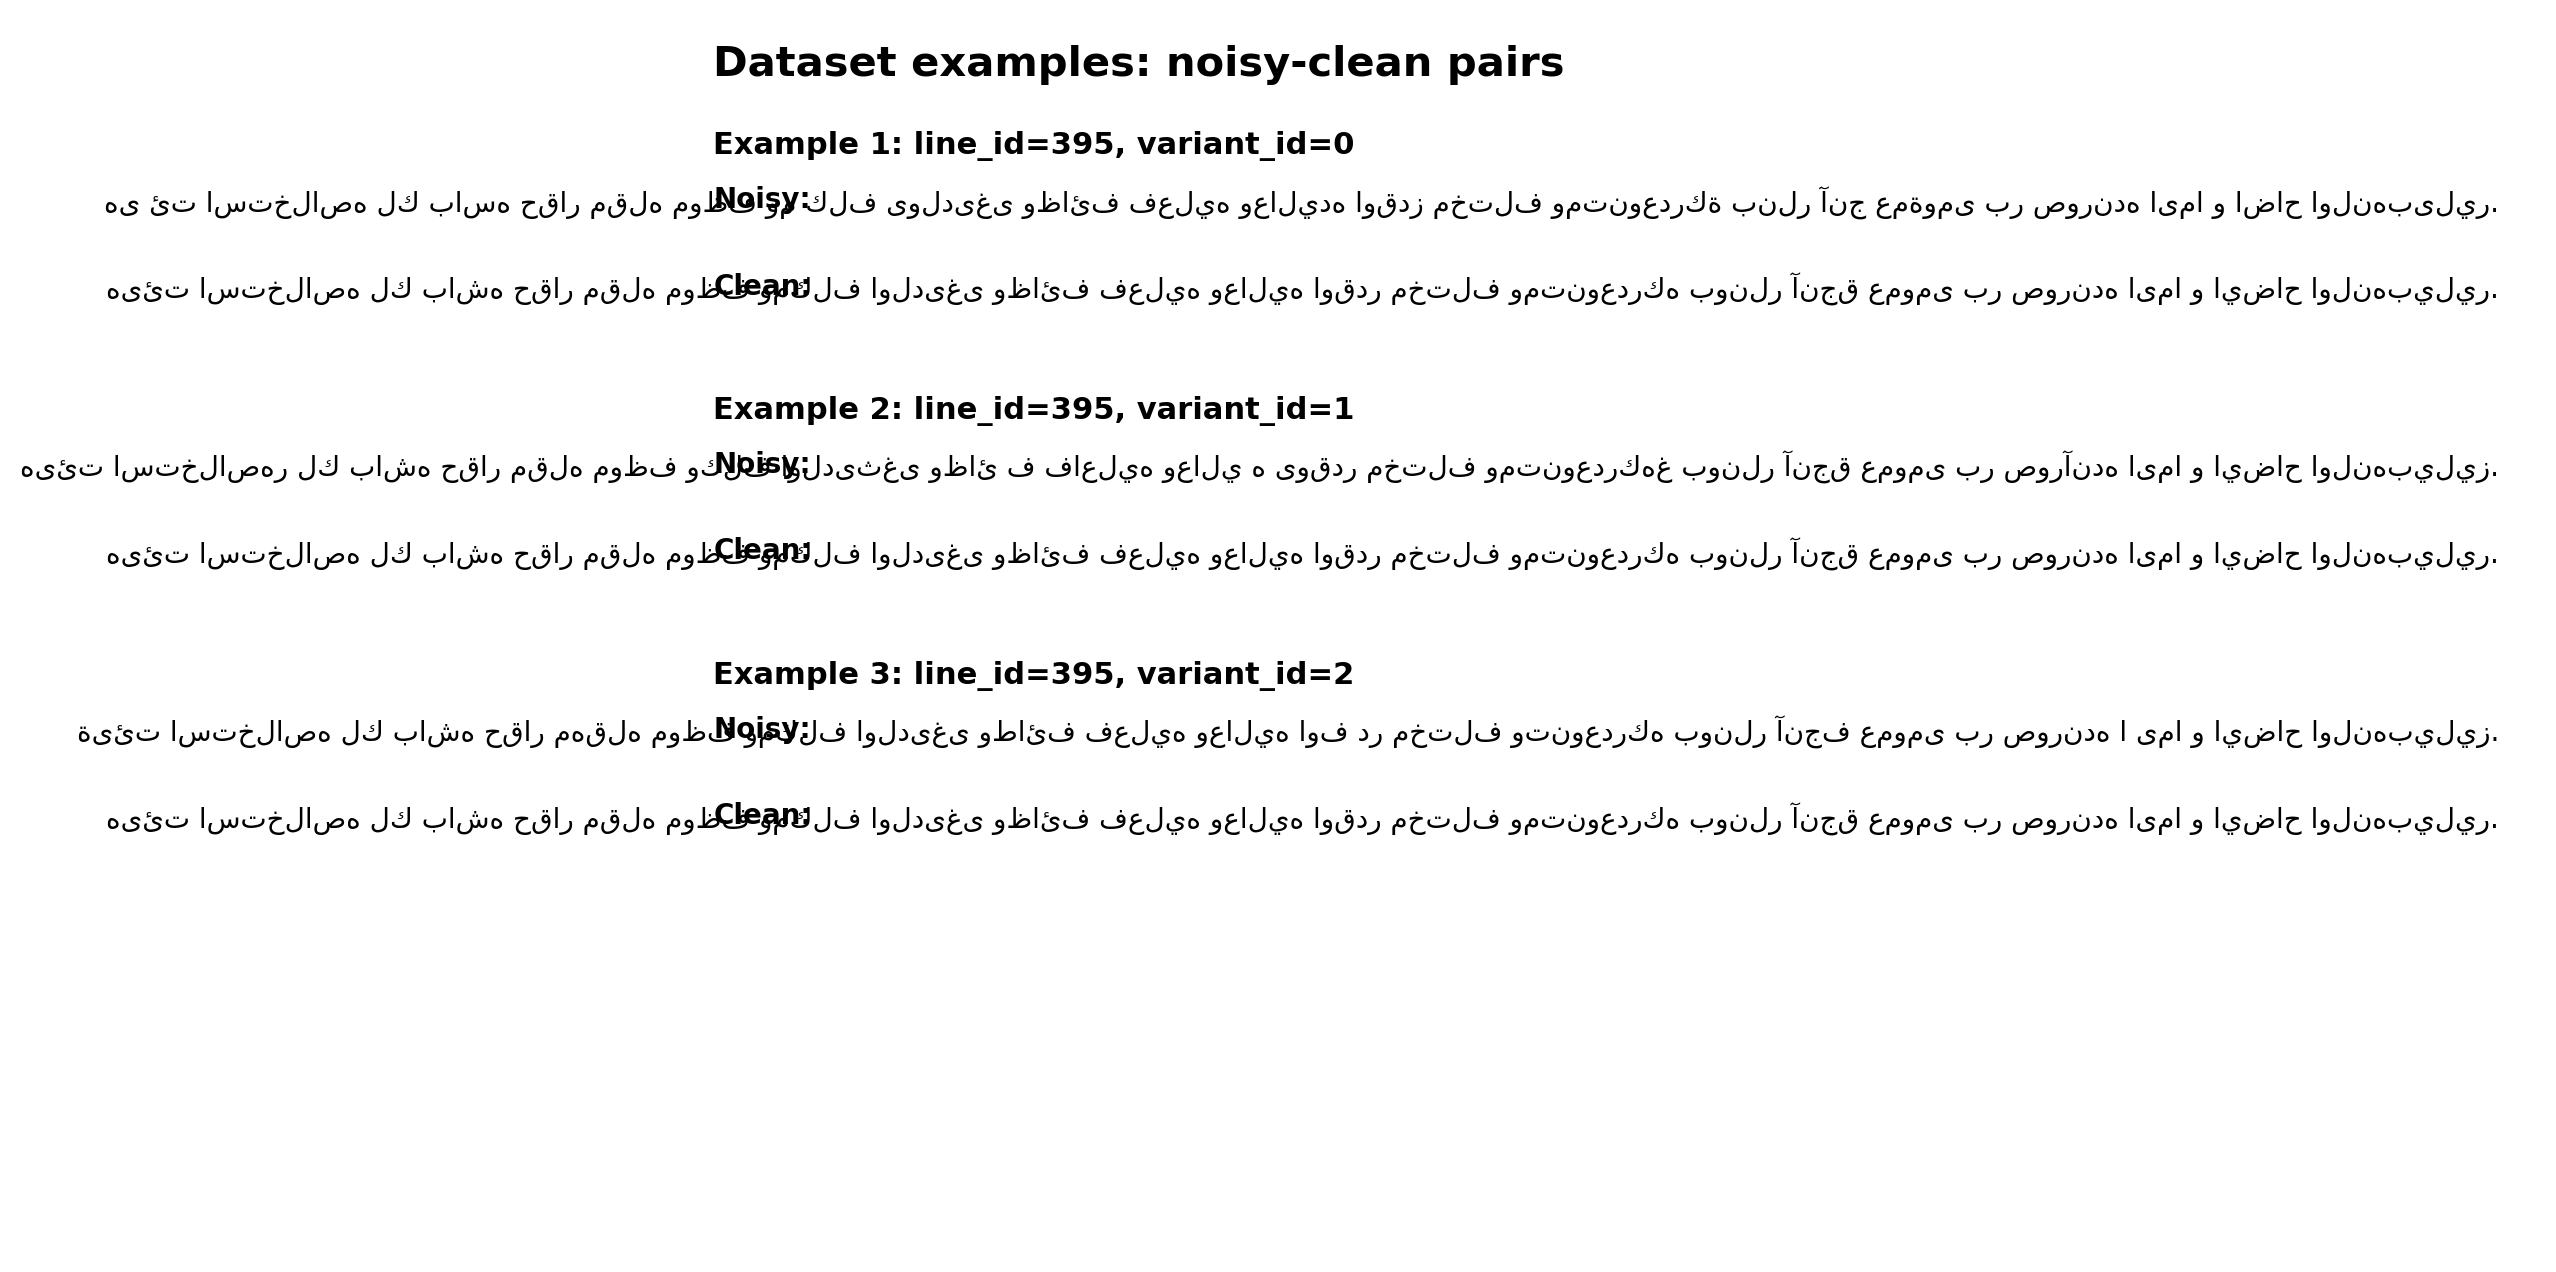
\includegraphics[width=\linewidth]{figures/dataset_examples.png}
    \caption{Examples of synthetic noisy-clean pairs from the test split.}
    \label{fig:dataset-examples}
\end{figure}


\section{Experiments}

\subsection{Metrics}

We use three metrics: Character Error Rate (CER), Word Error Rate (WER), and Exact Match.

CER is computed as:
\[
CER = \frac{S + D + I}{N},
\]
where $S$ is the number of substitutions, $D$ is the number of deletions, $I$ is the number of insertions, and $N$ is the number of characters in the reference text.

WER is computed analogously at the word level:
\[
WER = \frac{S_w + D_w + I_w}{N_w}.
\]

Exact Match is the fraction of examples where the predicted line exactly matches the clean reference line.

\subsection{Experiment Setup}

The benchmark contains train, validation and test splits. The final evaluation is performed on the test split. The identity and rule-based baselines are evaluated directly on the test set. The ByT5-small model is fine-tuned on the training split and evaluated on the test split.

The final ByT5-small configuration uses 512-token source and target sequence lengths and 2 training epochs. The main results are stored in \texttt{outputs/postcorrection/final\_metrics.csv}.

\subsection{Baselines}

The project includes two baselines. The identity baseline leaves noisy text unchanged. The rule-based normalizer applies simple Arabic-script normalization rules. These baselines are necessary because there is no previous published result on the proposed benchmark.

\section{Results}

\begin{table}[tbh!]
\begin{center}
\begin{tabular}{lrrrr}
\toprule
Method & CER $\downarrow$ & WER $\downarrow$ & Exact Match $\uparrow$ & N \\
\midrule
Identity baseline & 0.086005 & 0.519006 & 0.001250 & 800 \\
Rule-based normalizer & 0.151932 & 0.684408 & 0.000000 & 800 \\
Train-derived char-confusion baseline & 0.082520 & 0.506189 & 0.001250 & 800 \\
\textbf{ByT5-small 512 / 2 epochs} & \textbf{0.079913} & \textbf{0.368540} & \textbf{0.003750} & 800 \\
\bottomrule
\end{tabular}

\caption{Main test results on the proposed benchmark. Lower CER and WER are better; higher Exact Match is better.}
\label{tab:results}
\end{center}
\end{table}

The ByT5-small 512-token model achieves the best CER and WER among the evaluated methods on the proposed benchmark. The rule-based normalizer performs worse than the identity baseline. This suggests that naive normalization can distort meaningful orthographic properties of historical Arabic-script Turkic text.

The improvement is stronger for WER than for CER. This indicates that the model often repairs word-level structure even when exact character-level recovery remains difficult. Exact Match remains low for all methods because the lines are long and orthographically complex.

\subsection{Error Analysis}

\begin{table}[tbh!]
\begin{center}
\begin{tabular}{lrrrr}
\toprule
Criterion & Improved & Unchanged & Worse & Total \\
\midrule
CER & 682 & 60 & 58 & 800 \\
WER & 677 & 63 & 60 & 800 \\
\bottomrule
\end{tabular}

\caption{Per-sample error analysis for ByT5-small 512 compared with the noisy input.}
\label{tab:error}
\end{center}
\end{table}

The error analysis shows that the model improves most test examples, but it is not uniformly safe. Some predictions are worse than the noisy input. Therefore, the model should be treated as a useful post-correction component rather than a fully automatic scholarly transcription tool.


\subsection{Qualitative Examples}

In addition to aggregate metrics, we inspected individual examples. Table~\ref{tab:qualitative} shows representative improved and degraded cases. The full Arabic-script noisy, predicted and clean strings are provided in \texttt{docs/nlp\_final/qualitative\_examples\_full.md}. The examples confirm that ByT5 often repairs local OCR-like distortions, but can also introduce harmful changes.

\begin{table}[tbh!]
\begin{center}
\small
\begin{tabular}{|r|l|r|r|p{0.46\linewidth}|}
\hline
Row & Case & $\Delta$CER & $\Delta$WER & Qualitative interpretation \\
\hline
254 & Improved & 0.097 & 0.400 & Repairs multiple OCR-like distortions and reduces both character-level and word-level error. \\
\hline
126 & Improved & 0.093 & 0.286 & Repairs multiple OCR-like distortions and reduces both character-level and word-level error. \\
\hline
582 & Improved & 0.087 & 0.364 & Repairs multiple OCR-like distortions and reduces both character-level and word-level error. \\
\hline
384 & Worse & -3.937 & -4.417 & Introduces additional changes; this supports the limitation that neural post-correction is not uniformly safe. \\
\hline
392 & Worse & -3.810 & -4.167 & Introduces additional changes; this supports the limitation that neural post-correction is not uniformly safe. \\
\hline
\end{tabular}

\caption{Representative qualitative examples for ByT5-small 512. Positive $\Delta$ values mean improvement over the noisy input.}
\label{tab:qualitative}
\end{center}
\end{table}


\section{Limitations}

The current benchmark is intentionally limited. First, the corpus is small and comes from one main source. Second, the noisy-clean pairs are based on synthetic OCR-like corruptions rather than real OCR or HTR outputs. Third, the model is evaluated automatically and has not yet been validated by a domain expert. Finally, some ByT5 predictions are worse than the original noisy input, so the model should be used as an assistive post-correction component rather than a fully automatic scholarly transcription system.

\section{Conclusion}

This project introduced a reproducible pilot benchmark for OCR post-correction of low-resource Arabic-script Turkic historical text. We collected a small clean corpus, generated synthetic OCR-like noisy-clean pairs, created a train/validation/test split without clean-line leakage, and compared identity, rule-based and ByT5-small approaches.

The ByT5-small 512-token configuration achieved the best CER and WER among the evaluated methods on the proposed benchmark. At the same time, the experiment has important limitations: the corpus is small, the current data comes from one main source, errors are synthetic, and real OCR/HTR outputs should be added in future work. The project therefore represents a reproducible pilot study and a foundation for future work rather than a finished OCR system.

\bibliographystyle{apalike}
\bibliography{lit}

\end{document}
